\section{Exercise 5}
For this problem we will focus on solving the non-dimensional steady-state
heat transfer equation. Starting with the general heat transfer equation,
namely
\begin{equation}
    \rho c_{p} \pdv{T}{t} = k \pdv{T}{x}{x} + \dot{Q}
    \label{eq:heat-transfer}
\end{equation}
where $\rho$ is the density, $c_{p}$ is the specific heat, and $k$ is the
thermal conductivity. Next, we can properly non-dimensionalize
Eq.~(\ref{eq:heat-transfer}) to get the following 
\begin{equation}
    \pdv{T}{t} = \pdv{T}{x}{x} + \dot{Q}
    \label{eq:non-dim-heat-transfer}
\end{equation}
where the left hand side represents the unsteady terms, the first term on
the right hand side represents the diffusive transport of energy, and the
last term contains the source and sink terms. Furthermore, for steady-state
problems, like the one we are interested in,
Eq.~(\ref{eq:non-dim-heat-transfer}) further reduces to
\begin{equation}
    \dv[2]{T}{x} = - \dot{Q}
    \label{eq:heat-ode}
\end{equation}
Next, we can apply Eq.~(\ref{eq:heat-ode}) to the control volume shown in
Fig.~(\ref{fig:control-volume}). The control volume shows a solar water
heater that draws water from a well at temperature $T_{w} = 10$
(non-dimensional), and uses the thermal flux from the sun given as
$\dot{Q}=50\sin(2 \pi x)$ to heat up water to temperature $T_{in} = 50$.
Performing a control volume analysis we get the following ordinary
differential equation,
\begin{subequations}
    \begin{equation}
        \dv[2]{T}{x} = - \dot{Q}
        \label{eq:1d-heat-transfer-1}
    \end{equation}
    along with the following boundary conditions
    \begin{equation}
        T(x=0) = T_{w}
    \end{equation}
    \begin{equation}
        T(x=0) = T_{in}
    \end{equation}
    \label{eq:1d-heat-transfer}
\end{subequations}
\begin{figure}[H]
    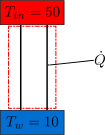
\includegraphics[height=2.5in]{../media/control-volume}
    \caption{Water heater exchanger}
    \label{fig:control-volume}
\end{figure}

\begin{enumerate}[label=(\alph*)]
    \item Start by discretizing Eq.~(\ref{eq:1d-heat-transfer-1}) using the
        second order central difference method
        \begin{equation}
            \dv[2]{f}{x} \approx
                    \frac{f_{i+1} - f_{i} + f_{i-1}}{\Delta x^{2}}
        \end{equation}
        and construct the coefficient and solution vectors (refer to pg. 21
        of Module 1). Show these matrices for a domain discretized with
        $M=8$ equidistant elements.    

    \item Solve Eq.~(\ref{eq:1d-heat-transfer}) using the tri-diagonal
        solver from the previous exercise on a mesh of $M=4, 8, 16, 32, 64$
        equidistant elements. Furthermore, compare the approximate solution
        obtained from the tri-diagonal solver to the exact analytical
        solution for each mesh. Please provide five plots with two curves
        comparing the results from the analytical and numerical solutions.
        Lastly, discuss your results.

    \item Conduct a performance study on your tri-diagonal solver by
        solving Eq.~(\ref{eq:1d-heat-transfer}) with $M=10, 100, 1000,
        5000, 10000$ elements and plotting mesh size versus time. Briefly
        discuss your results.

    \item Re-do parts (b) and (c), however instead of using your
        tri-diagonal solver, solve the system using 
        $T=\mathbf{A}^{-1}\mathbf{b}$. Briefly discuss your results,
        ensuring to compare the performance and accuracy between the two
        methods.
\end{enumerate}
